\section{Linguistic tools}

One of the main parts of Reprotool project is an automated analysis of the use case steps. This functionality saves user's work with tedious manual annotation - all the user has to do is to push a button. However, if user is not satisfied with results he can always manually tweak the analyzed use case step. This chapter describes implementation of linguistics analysis in Reprotool project and its linguistics background.

\subsection{Introduction}
Process of linguistic analysis gets natural language sentences as an input and returns analyzed usecases as is shown at figure \ref{fig:LinguisticsAnalyseSmall}. Whole process is divided into two parts: process of parsing and core analysis. Parsing contains main linguistic operations which are tokenization, tagging, parsing and lemmatization. Core work of parsing process is done by popular external linguistic analysis tools described in section \ref{sec:externaltools}. Core analysis converts parsed sentence trees with annotations into our usecases model. This process is described in more detail in section \ref{sec:analysis}. 

It is recommended to see section \ref{sec:analyzer}, where is also located our linguistic model at figure \ref{fig:ReprotoolLingModel}.

\begin{itemize}
\item {\bf Text preparation} Cleaning up input text and tokenization
\item {\bf Dependency trees} POS tagging and parsing
\item {\bf Constituents} determining important text ranges
\item {\bf Action type} final output result of analysis
\end{itemize}

Each implementation of any analyse brings problem of measuring success. We have put together a dataset of nearly three hundred sentences. These sentences contain the most common use cases operations. All these sentences were manually annotated and analyzed. In section \ref{sec:benchmark} is described our benchmark solution with actual results.

\begin{figure}[ht]
  \centering
  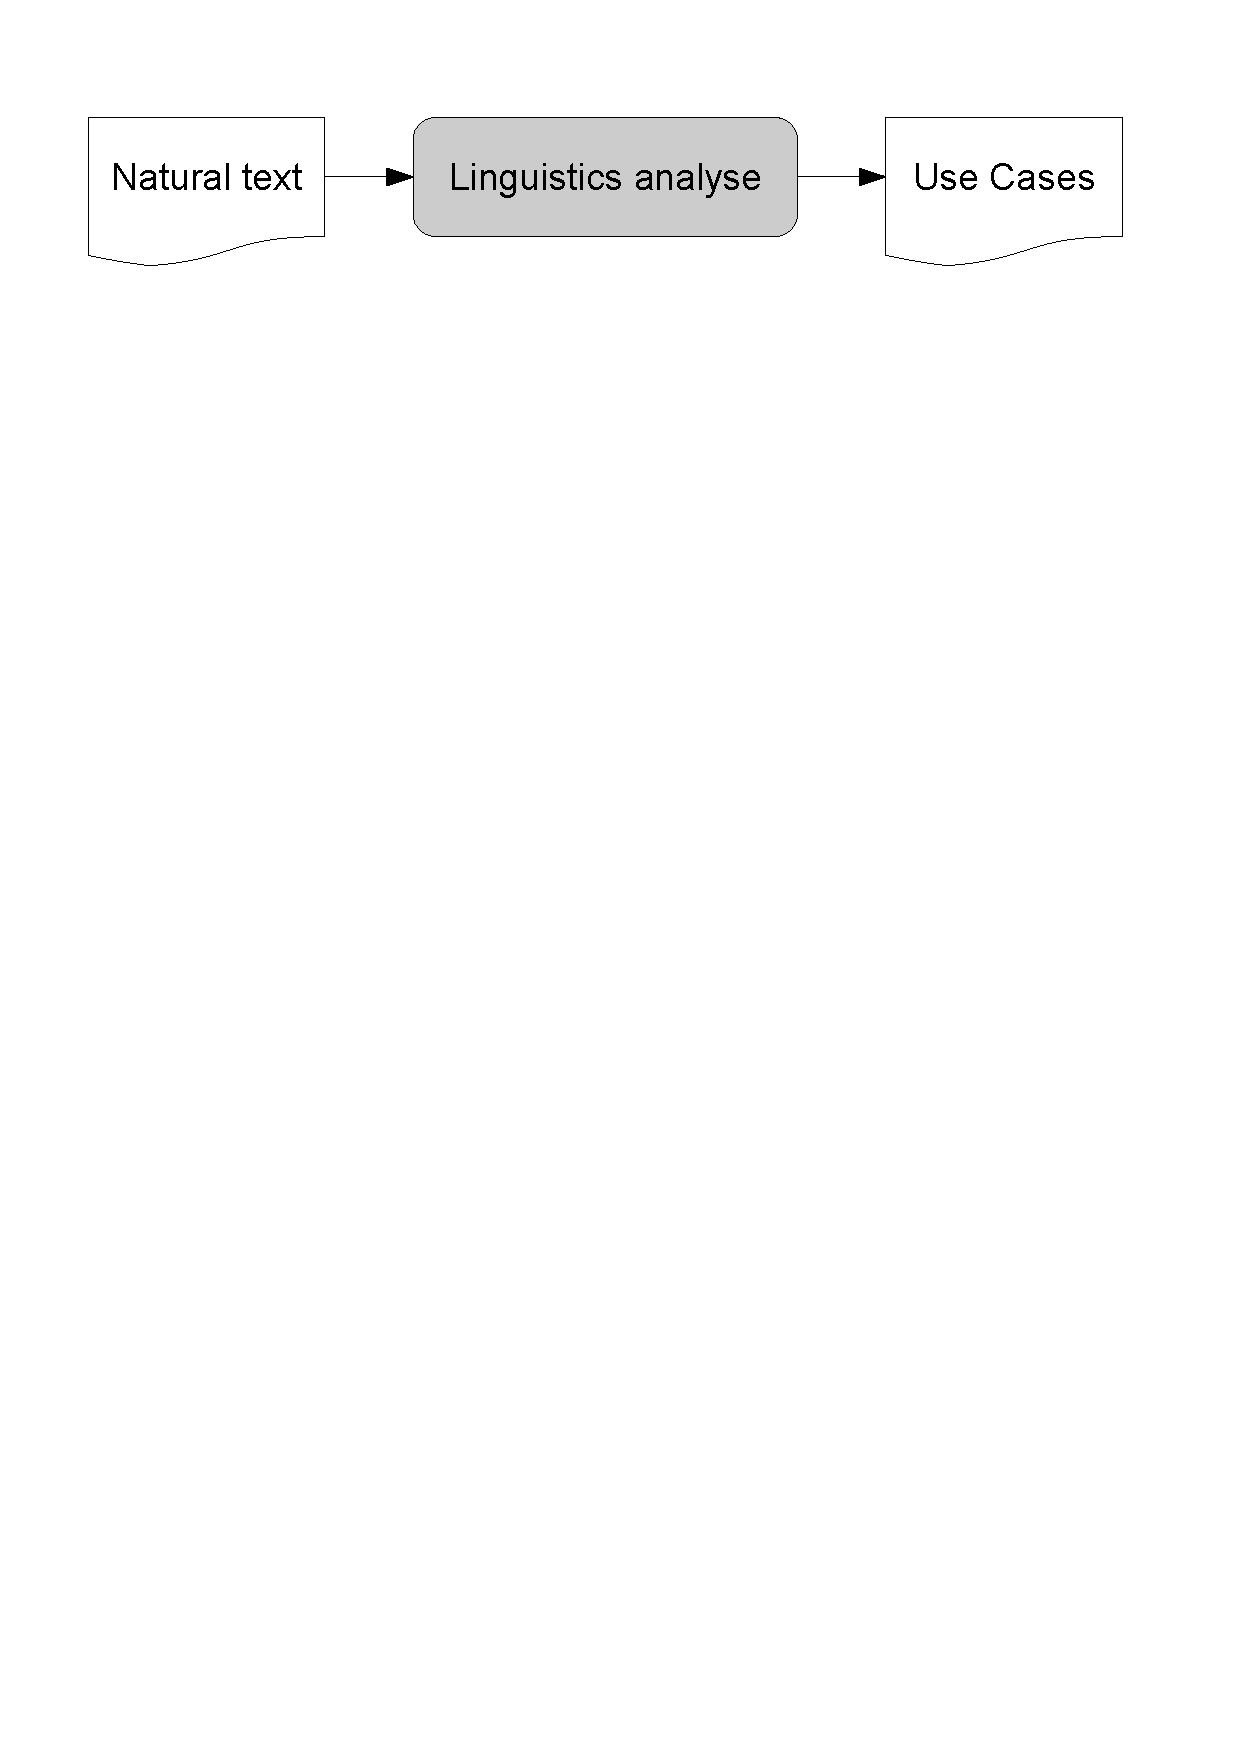
\includegraphics[height=30pt]{images/LinguisticsAnalyseSmall}
  \caption{Process of sentence analysis}
  \label{fig:LinguisticsAnalyseSmall}
\end{figure}

Following pages contain description of the used linguistics tools. All tools use Penn TreeBank tags notation. We use this notation in our model and our tools as well.

\subsection{External tools}
\label{sec:externaltools}
As described in previous sections whole process of linguistics analysis is not a trivial task. We chose commonly used external tools for some parts of analysis and bundled them as Eclipse plugins.

These parts were \emph{part-of-speech tagging}, \emph{sentence parsing} and \emph{obtaining lemma forms} for words. Main reasons for our selection were widespread usage and credibility of the tools, at least partial compatibility of output and input formats and Java implementation. 

We demanded Java implementation, because runtime control of programs written in different languages is inoperative and bring problems in portability of the project. The selected tools don't provide access to analysed entities in form of Java objects, but we are able to control their correct running.

Needed models for all tools are build and packed with bundles corresponding to these tools. These bundles are \verb|reprotool.tools.anna|,  \verb|reprotool.tools.dbparser| and \verb|reprotool.tools.mxpost|.


Selected tools are:
 
\begin{itemize}
\item {\bf MXPOST tagger} - \href{http://www.inf.ed.ac.uk/resources/nlp/local_doc/MXPOST.html}{Java implementation of well known Maximum Entropy Part-Of-Speech Tagger}
\item {\bf Dan Bikel's Multilingual Statistical Parsing Engine } - Java implementation coming from \href{http://www.cis.upenn.edu/~dbikel/software.html#stat-parser}{Dan Bikel’s Home Page}
\item {\bf Mate-tools lemmatizer} - part of bigger project called \href{http://code.google.com/p/mate-tools/}{Tools for Natural Language Analysis}
\end{itemize}

Larger list of tools could be found at project site. There are also links to similar pages concerned with the same theme. 
          
\subsubsection{MXPOST tagger} 
MXPOST tagger was written in Java implementation at University of Edinburg by NLP group and is maintained as part of theirs NLP tools.
        
Main part of this tagger is based on original parser written by Adwait Ratnaparkhi. Detailed description of this original parser is described in article \cite{Linguistics-ratnaparkhi96} and in his PhD thesis \cite{Linguistics-ratnaparkhi98}. 

Input data, natural language sentences, have to be tokenized according to the Penn Treebank conventions. Tagger needs for the run its model consisting of tagged data. Input data are then tagged with use of maximum entropy probability distribution. So the tagger has to find sentence with similar structure in the trained data.
  
\subsubsection{Dan Bikel's Multilingual Statistical Parsing Engine}   

Statistical parsing engine does two main tasks. First is creating and training of the model and second is core parsing. For these purposes we had to obtain large data model with parsed sentences. 

During the parsing, parser is trying to find the most similar sentence in trained model. As a trained data, we use a part of \emph{Penn Treebank, Wall Street Journal collection}.

\subsubsection{Mate-tools lemmatizer}          
          
This lemmatizer is working in a similar way like previous parser. It also needs similar data models, because it cannot use just list of lemmas and their word forms. It also needs to obtain POS information for correct work.

This tool uses one word per line 2009 CoNLL input format, so we had to divide our sentences to adapt them to this format.

\subsection{Linguistic analysis}
\label{sec:analysis}
Linguistics analysis covers multiple different actions executed by various tools. Connection of these tool is described at figure \ref{fig:LinguisticsAnalyse}. In this section are described only pure linguistic tools. Core structure of our action type determining analyzer is described in section \ref{sec:analyzer}.

All tools have at least our wrapper. This wrapper tries to keep selected tool running if possible. This speeds up analysis approximately ten times.

As you can see, this pipeline obtains structure similar to dependency tree for each sentence. We are storing for each sentence this dependency tree. For each word in sentence we also store POS tag and lemma form.

\begin{figure}[ht]
  \centering
  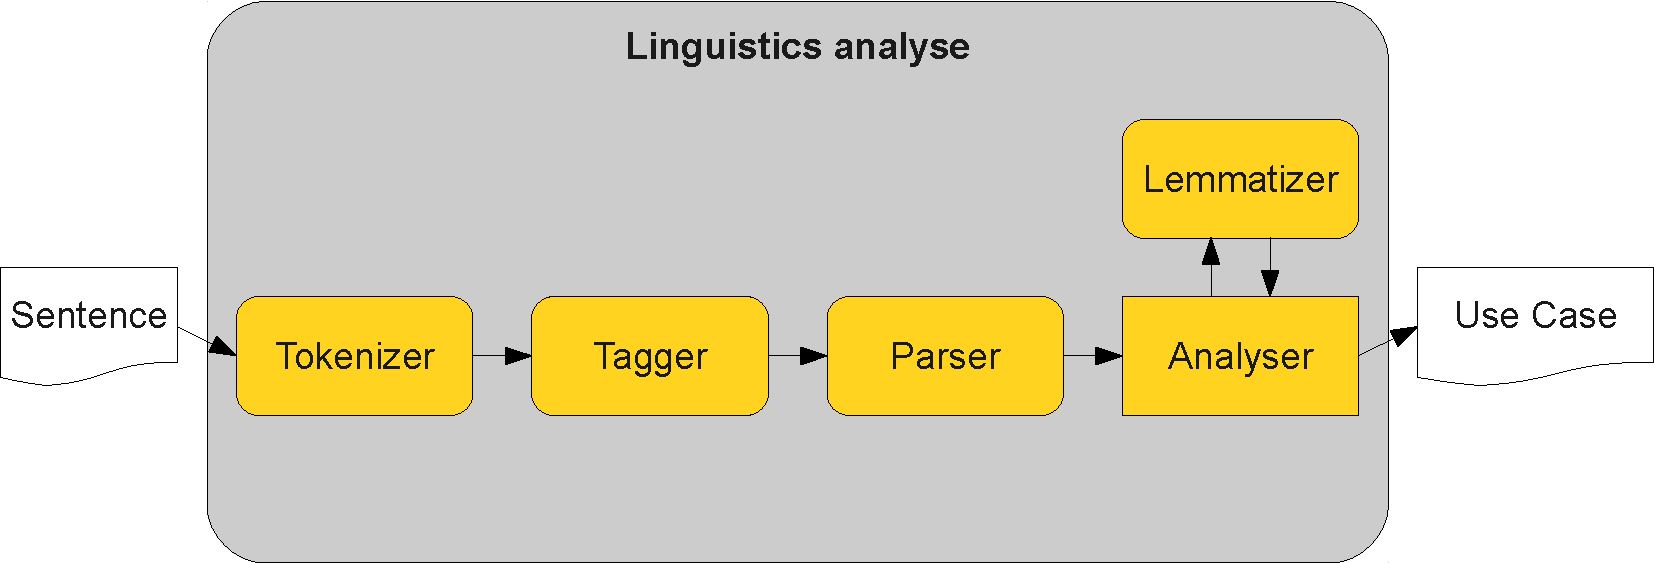
\includegraphics[width=400pt]{images/LinguisticsAnalyse}
  \caption{Process of sentence analysis}
  \label{fig:LinguisticsAnalyse}
\end{figure}

As we can see, the biggest problem is data conversion between two following tools. These important actions are described by input and output data of each task.

\subsubsection{Tokenization}
First part of natural language processing is provided by our own tokenizer. Tokenizer splits sentence into set of separated strings called tokens. These tokens are base units for natural language processing. Each token usually represents one word, a number or punctuation. Invalid tokens are striped by following tools, but these tools are not stripping parts of the tokens.

\begin{table}[ht]   % or b
\begin{center}
  \begin{tabular}{| r | l |}
\hline
Input 	&	Natural language sentence \\ \hline
Output &	Array of tokens (eg. words, numbers) \\ 
\hline
  \end{tabular}
  \caption{Tokenizer data formats}
  \label{tab.tokenization}
\end{center}
\end{table} 

    


\subsubsection{Tagging}
Tagging adds information for each word. Usually determines part of the speech, but it can also obtain more linguistic categories. We use external POS tagger and our analysis uses only POS information.

\begin{table}[ht]   % or b
\begin{center}
  \begin{tabular}{| r | l |}
\hline
Input 	& Array of tokens \\ \hline
Output 	& Array of POS tagged tokens (eg. adjectives, verbs) \\ 
\hline
  \end{tabular}
  \caption{Tagger data formats}
  \label{tab.tagging}
\end{center}
\end{table} 


\subsubsection{Parsing}
Main task of parser is creation of the dependency tree for each sentence. Parser determines all sentence parts and their types. It also sets their interdependences. For better explanation, example of parsed tree could be found at figure \ref{fig:ParsedTree}.

Our project uses external parser wrapped into Eclipse plugin. 


\begin{table}[ht]   % or b
\begin{center}
  \begin{tabular}{| r | l |}
\hline
Input 	& Array of POS tagged tokens \\ \hline
Output 	& Parse trees of each sentence \\ 
\hline
  \end{tabular}
  \caption{Parser data formats}
  \label{tab.parsing}
\end{center}
\end{table} 



\subsubsection{Lemmatization}
Lemmatization basically means finding lemma forms for all words in a sentence. As stated, we are using external tool for this purpose wrapped in Eclipse plugin.

\begin{table}[ht]   % or b
\begin{center}
  \begin{tabular}{| r | l |}
\hline
Input 	& Parse trees of each sentence \\ \hline
Output 	& Lemma for each word \\ 
\hline
  \end{tabular}
  \caption{Lemmatizer data formats}
  \label{tab.lemmatizer}
\end{center}
\end{table} 


\begin{figure}[ht]
  \centering
  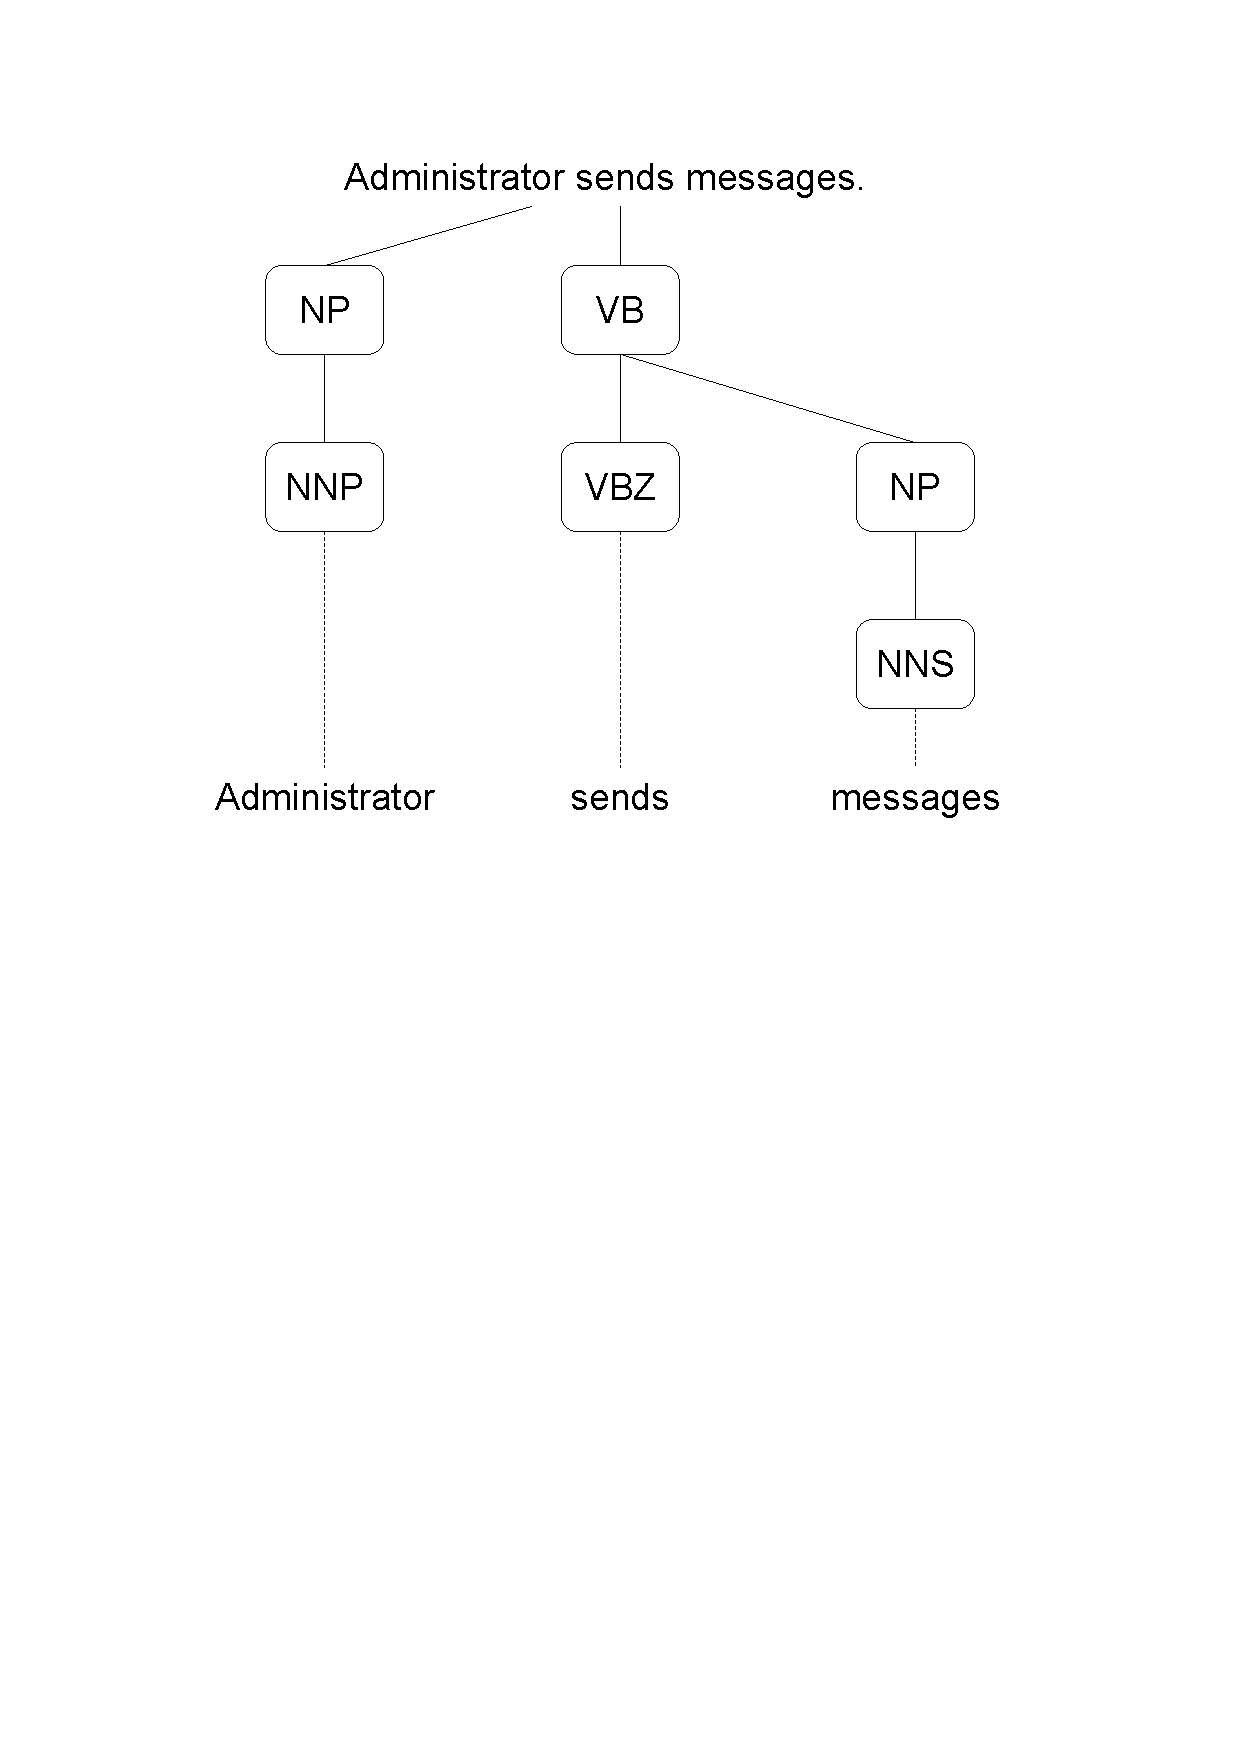
\includegraphics[width=200pt]{images/ParsedTree}
  \caption{Parsed tree of sentence "Administrator sends messages".}
  \label{fig:ParsedTree}
\end{figure}

\subsection{Analyzer}
\label{sec:analyzer}
This section contains two important parts. First is process of the whole linguistic analysis and the second is basic description of our core analyser.

\subsubsection{Analysis process}
This section contains description of set of all important analysis steps. We recommend to use this section as an entry point for reading \emph{Reprotool} source code.
Important linguistic model is shown at figure \ref{fig:ReprotoolLingModel}. 

First part of process is initialization. This process is executed at startup of \emph{Reprotool}:

\begin{itemize}
\item {\bf Initialize tagger} - external tagger is initialized.
\item {\bf Initialize parser} - external parser is initialized and started.
\item {\bf Initialize lemmatizer} External lemmatizer is initialized started.
\item {\bf Analysis of the initialization sentence} - this step speeds up following analyses by memory initialization.
\end{itemize}

Initialization process is executed as Eclipse job and should take about ten seconds (depending on infrastructure). If initialization faces error, it tries to restart.\\

Second, bigger part on analysis process is sentence analysis. Its start is triggered by user pushing a button in IDE ( analyze command for use case step or in loop for all use case steps in use case). This process contains following steps:

\begin{itemize}
\item {\bf Execute linguistic analysis job for one sentence} - runs all four linguistic tools for selected sentence. When tools encounter error, analysis is executed with safe version of sentence with stripped bad characters. 
\item {\bf Match sentence object} - at this point we have original sentence string and sentence object with dependency tree. We have to match these objects for final action type text ranges marking.
\item {\bf Find text ranges} - analyze sentence for apostrophes and quotation marks. This step improves label targeting.
\item {\bf Execute core analyzer} - determines constituents and action types.
\item {\bf Prepare model changes} - stacks all needed changes of model. Changes must be valid and must corresponds.
\item {\bf Return results to UI} - all changes to model are executed at one place by UI. UI has always control over internal model.
\end{itemize}

\subsubsection{Core analyzer}
Part of our project called "core analyzer" describes process following basic linguistic analysis. This core analyzer accomplish two main tasks:

\begin{itemize}
\item {\bf Determine constituents} - find all important words in sentence.
\item {\bf Determine action type} - set final action type.
\end{itemize}

Rules for determining constituents are described in own section \ref{sec:lingbackground}. Constituents are determined in order: subject, main verb, indirect object, representative object.

Also action types have own section \ref{sec:actiontypes}. These types are determined in order: Include, Goto, Abort, Internal, To system, From system. Rules for last three types are mostly used at same time.

All changes made by core analyzer are stored in \verb|CompoundCommand| object. Therefore, all changes are made at one place an user can undo these changes.

\begin{figure}[ht]
  \centering
  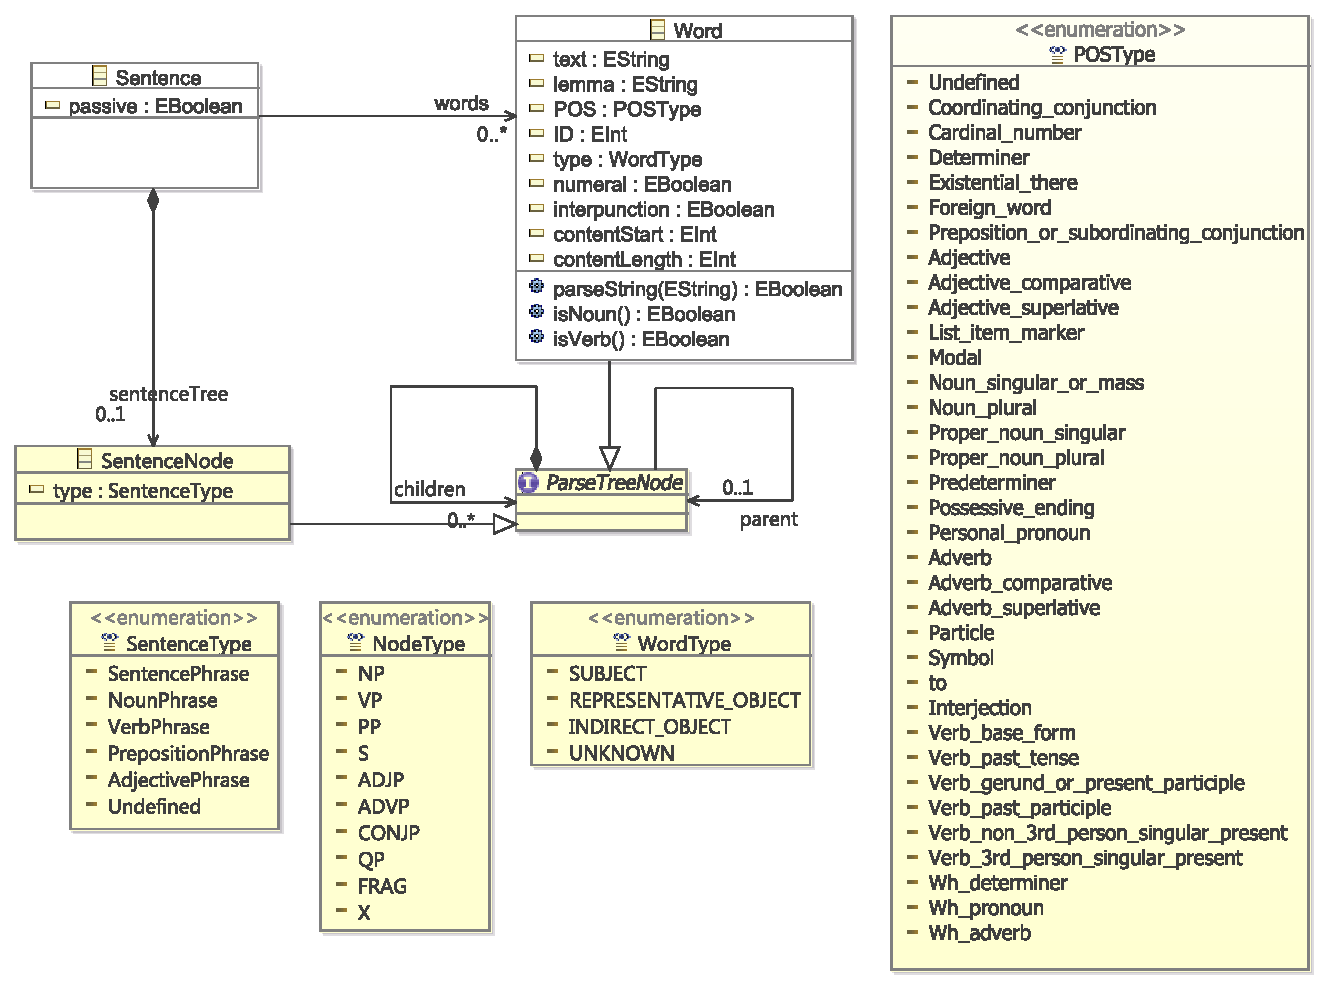
\includegraphics[width=\textwidth]{images/ReprotoolLingModel}
  \caption{Internal linguistics model with enumerations.}
  \label{fig:ReprotoolLingModel}
\end{figure}

\subsection{Linguistics constituents background}
\label{sec:lingbackground}
Main goal of linguistic analysis in our project is to identify important words in a sentence. These words are mainly constituents. For our purpose, we are identifying four groups of words:

\begin{itemize}
\item {\bf Subject} main subject of the sentence
\item {\bf Main verb} verb which specifies meaning
\item {\bf Representative object} main subject of sentence action
\item {\bf Indirect object} an actor to whom or for whom the action of the verb is done and who is receiving the \emph{Representative object}
\end{itemize}

These words are used in action analysis. We are matching sentences to proper actions with a set of deriving rules, which are based on these words. 
                                                                    
\subsubsection{Subject}
For our purpose, subject must be always an actor. User has to add sentence actors before analysis. Usually is subject noun in a top noun phrase. If the sentence is in passive, subject stands at object's place. 

Subject could be also missing. In that case analysis still tries to find other constituents.

There are two predefined actors, "system" and "user". Automatic analysis uses these actors, but it is strongly recommended, that user adds these actors to project.

\subsubsection{Main verb}
This verb is a main verb of highest verb phrase in a sentence. In a passive sentence is auxiliary verb ignored. 

Finding verb in properly parsed sentence is an easy task, but in a sentence with a wrong parsed tree it usually can not be resolved. It happens usually when parser doesn't know contained verb. This means, that parser tags verb by different POS tag.

\subsubsection{Indirect object}
Indirect objects are derived before representative (conceptual) objects. All indirect objects are actors and indirect objects aren't in the same node with other objects.

Node with indirect objects must be a noun phrase containing verb phrase. If this node is found, all objects are marked as indirect. Indirect object cannot be in possessive form.  

\subsubsection{Representative object}
Representative object could be noun in a noun phrase which is a child of main verb phrase. Except noun phrase with indirect objects.

If a phrase contains more nouns without conjunction, we mark as an object last of the nouns. This rule was established, because external tools usually determine adverbs as nouns. After all, noun with multiple adverbs still represents one object.

\subsection{Action types deriving rules}
\label{sec:actiontypes}
When we have determined all constituents, analysis can continue with determining proper action type. This is followed by filling internal models with obtained data from analysis. Each action type has its own set of deriving rules and these rules are strictly disjunct. This means, that only one action type can be assigned to analyzed sentence. This section contains description of these deriving rules. 

\subsubsection{Include use case action}
Sentence contains one of the following verbs: "continue", "repeat", "resume", "retry" and "include".  This verb must be main verb of the sentence. It also has to contain reference to usecase and label of one existing usecase in current project.

\subsubsection{Goto action}
Sentence contains one of the verbs from \emph{Include use case action}. This verb must be main verb of the sentence. In addition, target of the action must be found and it has to be existing use case step in current use case. 

\subsubsection{Abort action}
Set of abort verbs contains "abort", "terminate", "end", "exit" and "finish".  This verb must be main verb of the sentence.

\subsubsection{From system action}
System is the subject of the sentence and we have identified indirect object (other than system). System is communicating with other actor.

\subsubsection{To system action}
System is an indirect object. Subject cannot be system. Example of \emph{To system} action could be found at figure \ref{fig:ToSystemActionExample}. In common use case, this action type represents communication from subsystems to system.

\subsubsection{Internal action}
System is a subject and there is no indirect object, or system is also indirect object. This action type is used for majority of common system actions, like sending messages or throwing errors.

\begin{figure}[ht]
  \centering
  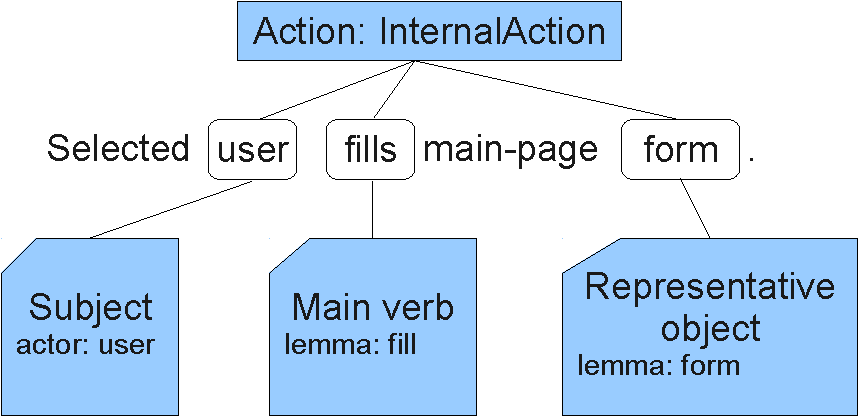
\includegraphics[width=250pt]{images/ToSystemActionExample}
  \caption{Example of To system action analysis result.}
  \label{fig:ToSystemActionExample}
\end{figure}

\subsubsection{Unknown action}
This is an default action type. If analysis could not find any other action, we set Unknown action type. This action type is also used when automatic analysis encountered error. 

\subsection{Benchmark}
\label{sec:benchmark}

We needed bigger set of proper sentences during the implementation of automatic linguistic analysis. These sentences were used for common testing purposes. Growing complexity of \emph{Reprotool} model demanded more and more testing sentences. Creation of own independent testing tool was just a logical step.

We have created special benchmark plug-in. This plug-in complement JUnit tests used during implementation and is part of {\tt reprotool.ling.tests} bundle. Core function of this plug-in is batch sentence analysis. Benchmark contains three main parts:

\begin{itemize}
\item {\bf Loading} - reading file containing annotated dataset.
\item {\bf Analysis} - batch analysis of all sentences in dataset.
\item {\bf Results output} - computing main results in usable format.
\end{itemize}

Our benchmark plug-in is ready to use. Usage of its features needs almost no source code modification. User only has to specify dataset file location. For quick run of this benchmark locate JUnit tests in {\tt reprotool.ling.tests} bundle and change noted dataset file location. Default location is set to file "data.csv" located in bundle.

Right usage of our benchmark plug-in is described in following list. This process is composed of more nontrivial tasks, but these tasks are easy to resolve.

\begin{enumerate}
\item {\bf Reprotool initialization} You have to be able successfully build our \emph{Reprotool} project. It is supposed, that user modifying our project is able to build Eclipse plug-in projects.
\item {\bf Obtaining sentences} First part of dataset creation is collecting data. It is recommended to obtain sentences from use cases.
\item {\bf Manual annotation} The most time consuming part is dataset annotation. Example of dataset file is located in table \ref{tab.benchmarkinput}.
\item {\bf Dataset location} User has to specify dataset location in source code.
\item {\bf Benchmark running} The easiest way to run benchmark is to execute corresponding JUnit test.
\end{enumerate}

Obtaining of proper dataset is more described in section \ref{sec:dataset}. 

\subsubsection{Implementation}
Benchmark plug-in uses same core functions like common \emph{Reprotool} linguistic analysis. Implementation of benchmark is slightly different from common analysis, because of data conversion an reading. We defined just two benchmark objects. First, main object, represents whole benchmark. Second object represents small version of one project. This small version of project comes from one dataset sentence. This means, that benchmark creates one project for each sentence. Main object contains list of these objects.

This difficult description could be better explained by following process. This process describes lifetime of one benchmark.

\begin{enumerate}
\item {\bf Main benchmark object is initialized} This step just sets up benchmark base properties,for example location of dataset.

\item {\bf Benchmark loads dataset} Benchmark locates dataset and in loop creates small project object for each sentence.
    \begin{enumerate}
    \item {\bf Loading sentence} Sentence with annotation is parsed. Representative results are created from annotation.
    \item {\bf Creating project} Benchmark creates project due to \emph{Reprotool} model. Benchmark sets up project, UseCase, Scenario, UseCaseStep and other needed objects.
    \item {\bf Linking objects} Benchmark links all objects, so the loaded sentence is not different from common UseCaseStep sentence.
    \end{enumerate}

\item {\bf Analyzing sentences} Benchmark analyzes each input sentence (now project)  like common project.
    \begin{enumerate}
    \item {\bf Linguistic tools} Parsed tree is created for each sentence.
    \item {\bf Action type} Analyzer tries to determine UseCaseStep action type.
    \item {\bf Store results} Important results are stored for each sentence.
    \end{enumerate}
\item {\bf Computing benchmark results} Benchmark computes final results from whole dataset. These results are printed to console. Example benchmark output is shown in table \ref{tab.benchmarkexample}.
\item {\bf Benchmark cleanup} Destruction of objects and termination.
\end{enumerate}

The most important part of benchmark are final results and their format. Result are computed for each annotated entity. Results for each entity consists of overall string. For example "{\tt OBJECTS: Count: 21 Found: 11 | 52,4\%}". This line is usually followed with set of lines containing errors. Each line starts with sentence identification, input (annotated) result and  output (analyzed) result. These informations are very important for localizing differences between input and output results.

Based on these informations, \emph{Reprotool} model can be changed for modified usage of our project to suit your needs.

\begin{table}[ht]   % or b
\begin{center}
    \begin{verbatim}
SUBJECTS: Count: 21 Found: 19 | 90,5%
RPT6: in-subjectNumber: 6 out-subjectNumber: 1
MOD1_UC1_7: in-subjectNumber: 0 out-esubjectNumber: 3
VERBS: Count: 21 Found: 20 | 95,2%
MOD1_UC1_5: in-verbLemma: "verify" out-verbLemma: "be"
INDIRECT_OBJECTS: Count: 21 Found: 20 | 95,2%
LING2: in-indirectObjectNumber: 8 out-indirectObjectNumber: 0
OBJECTS: Count: 21 Found: 11 | 52,4%
RPT8: in-objectNumber: 2 out-objectNumber: 0
LING1: in-objectNumber: 8 out-objectNumber: 4
MOD1_UC1_7: in-objectNumber: 3 out-objectNumber: 0
MOD1_UC1_8: in-objectNumber: 0 out-objectNumber: 5
TOTAL: Count: 84 Found: 70 | 83,3%   
    \end{verbatim}
  \caption{Example output from benchmark plugin}
  \label{tab.benchmarkexample}
\end{center}
\end{table}   
      
      
\subsubsection{Dataset}
\label{sec:dataset}
Most important precondition for benchmarking is good properly annotated dataset. In this section we would like to describe our annotation. It is recommended to see our annotated dataset before creation of other dataset.

We have defined eight basic sentence entities to annotate. These list could be followed with action type parameters. First entity is sentence identification string. This string is used for referencing to sentences, so it should be unique string for each sentence.

Entities are described in the following list:

\begin{enumerate}
\item {\bf ID } Id string for one sentence provided for sentence identification
\item {\bf SENTENCE } Test sentence
\item {\bf ACTORS } List of sentence actors (separated by commas)
\item {\bf SUBJECT\_NUMBER } Word index of subject
\item {\bf VERB\_LEMMA } Lemma form of main verb in a sentence
\item {\bf OBJECT\_NUMBER} List of objects indices
\item {\bf INDIRECT\_OBJECT\_NUMBER} Index of indirect objects (all indirect objects are in same sentence tree node)
\item {\bf ACTION\_CODE} Code of sentence action (sentence action type codes are described lower). 
\item {\bf ACTION\_PARAM1} First parameter of an action
\end{enumerate}   
   
There are few basic advices for annotation. All indices are starting from value 1. Value 0 indicates missing entity. Empty string in action code indicates Unknown action type. 

As mentioned in previous section, we have defined several action types. Each type should be also set in benchmark dataset. Defined action codes for corresponding action types are:      
     
\begin{itemize}
\item {\bf INTERNAL} Internal action
\item {\bf FROM\_SYSTEM} From system action
\item {\bf TO\_SYSTEM} To system action
\item {\bf GOTO} Continue action (parameter is an UseCaseStep)
\item {\bf ABORT} Abort use case action
\item {\bf INCLUDE} Include action (parameter is an UseCase)
\item {\bf UNKNOWN} Undefined action
\end{itemize}     

Table \ref{tab.benchmarkinput} contains few annotated sentences. You can see that annotation covers main results of common UseCaseStep analysis. And this is exactly the main purpose of our dataset annotation.
      
\begin{table}[ht]   % or b
\begin{center}
    \begin{scriptsize}  
    \begin{verbatim}      
ID;SENTENCE;ACTORS;SUBJECT_NUMBER;VERB_LEMMA;OBJECT_NUMBER;INDIRECT_OBJECT_NUMBER;ACTION_CODE;
_ ACTION_PARAM1;ACTION_PARAM2
RPT1;User opens window.;;1;open;3;;TO_SYSTEM;;
RPT2;System creates a new object.;;1;create;5;;INTERNAL;;
RPT3;User fills login.;;1;fill;3;;TO_SYSTEM;;
MOD1_UC1_5;System verifies if data is correct .;;1;verify;4;;INTERNAL;;
MOD1_UC1_6;System informs that account has been created .;;1;inform;4;;INTERNAL;;
MOD1_UC1_7;Some obligatory fields were not filled.;;0;be;3;;INTERNAL;;
MOD1_UC1_8;Systems highlights the missing fields .;;1;highlight;5;;INTERNAL;;
MOD1_UC1_9;Back to step 4 .;;0;;4;;GOTO;4;
    \end{verbatim}
    \end{scriptsize}
  \caption{Example input for benchmark plug-in}
  \label{tab.benchmarkinput}
\end{center}
\end{table}      
      
Main part of our benchmark dataset was obtained from \href{http://www2.put.poznan.pl/en}{Poznan University of Technology}, their \href{http://www.se.cs.put.poznan.pl/knowledge-base/software-projects-database/use-cases-database-ucdb/use-cases-database-ucdb}{Use Cases Database (UCDB)} and it coverts one project "\href{http://ucdb.cs.put.poznan.pl/benchmark/2.f.n/srs/index.html}{Admission System version 2.0F (quantitative)}".  

Whole dataset contains 269 manually annotated sentences. This dataset could be used for better use case verification, e.g. for benchmarking in any other project.   

\subsubsection{Results}
Our benchmark plug-in provides computed results after each execution. Obtaining results for other set of annotated sentences is very easy. There is no need to post-process benchmark results in any way.

Actual benchmark results of dataset analysis are shown in table \ref{tab.benchmarkresults}. shows current benchmark results. Total result is 88,10\%. This number means, that 11,90\% of tagged entities is not correctly recognized.

\begin{table}[ht]   % or b
\begin{center}
\begin{tabular}{l r r r}
 & Count & Found & Result \\
\hline
SUBJECTS: & 269 & 249 & 92,57\% \\
VERBS: & 269 & 244 & 90,71\% \\
INDIRECT OBJECTS:& 269 & 260 & 96,65\% \\   
OBJECTS: & 269 & 200 & 74,35\% \\
ACTIONS: & 269 & 232 & 86,25\% \\
\hline
TOTAL: & 1345 & 1185 & 88,10\% \\
\hline
\end{tabular}

  \caption{Final benchmark results}
  \label{tab.benchmarkresults}
\end{center}
\end{table}    
 
As you can see, our analysis returns result corresponding to manual annotation in 88,10\% of all cases. This number also means, that 11,90\% of tagged entities is not correctly recognized.

Results also show accuracy of selected analysis subtasks. We have to remind, that reference results were provided by our manual annotation. It is not too difficult to obtain own, more independent results. Annotators have to only follow instructions in previous section.

